
          %-------------------------------------%
\chapter{~~Progressive mesh generation; knitting}\label{\numb section 3}
          %-------------------------------------%

Section \ref{\numb section 2} shows how to build meshes by joining together several regular meshes
(triangles or quadrangles), like patches.
The present section explains how to build a mesh by gradually adding cells, on by one.
We call this approach ``progressive mesh generation''.
In some cases, the process starts with a given interface and adds triangles, one by one,
moving and deforming the interface, until it shrinks and disappears.
In some cases (like in paragraphs \ref{\numb section 3.\numb parag 2},
\ref{\numb section 3.\numb parag 4}, \ref{\numb section 3.\numb parag 6},
\ref{\numb section 3.\numb parag 7}) we begin with nothing at all;
{\maniFEM} finds a starting point by itself.

Progressive mesh generation works with segment cells (for one-dimensional meshes) and
triangular cells (for two-dimensional meshes).
Meshing of three-dimensional domains will be implemented in the future and will use tetrahedral
cells.

Progressive mesh generation follows the shape of the current working manifold (the most recently
declared {\small\tt \verm{Manifold}} object) by {\small\tt project}ing each newly constructed vertex
on that manifold.
Recall that in this manual we use the term ``manifold'' to mean a manifold without boundary.


          %--------------%
\section{~~Filling a disk}\label{\numb section 3.\numb parag 1}
          %--------------%

Paragraph \ref{\numb section 2.\numb parag 9} shows how to build a mesh over a disk,
but the quality of the mesh is quite poor.
This is so because the {\small\tt \verm{Mesh}} constructor with {\small\tt \verm{tag}::quadrangle} treats the
disk as a (much) deformed rectangle.

We can ask {\maniFEM} to progressively mesh the disk, starting from its boundary (a circle)
and adding triangles, one by one, until the disk is completely covered :

\begin{figure} \centering
 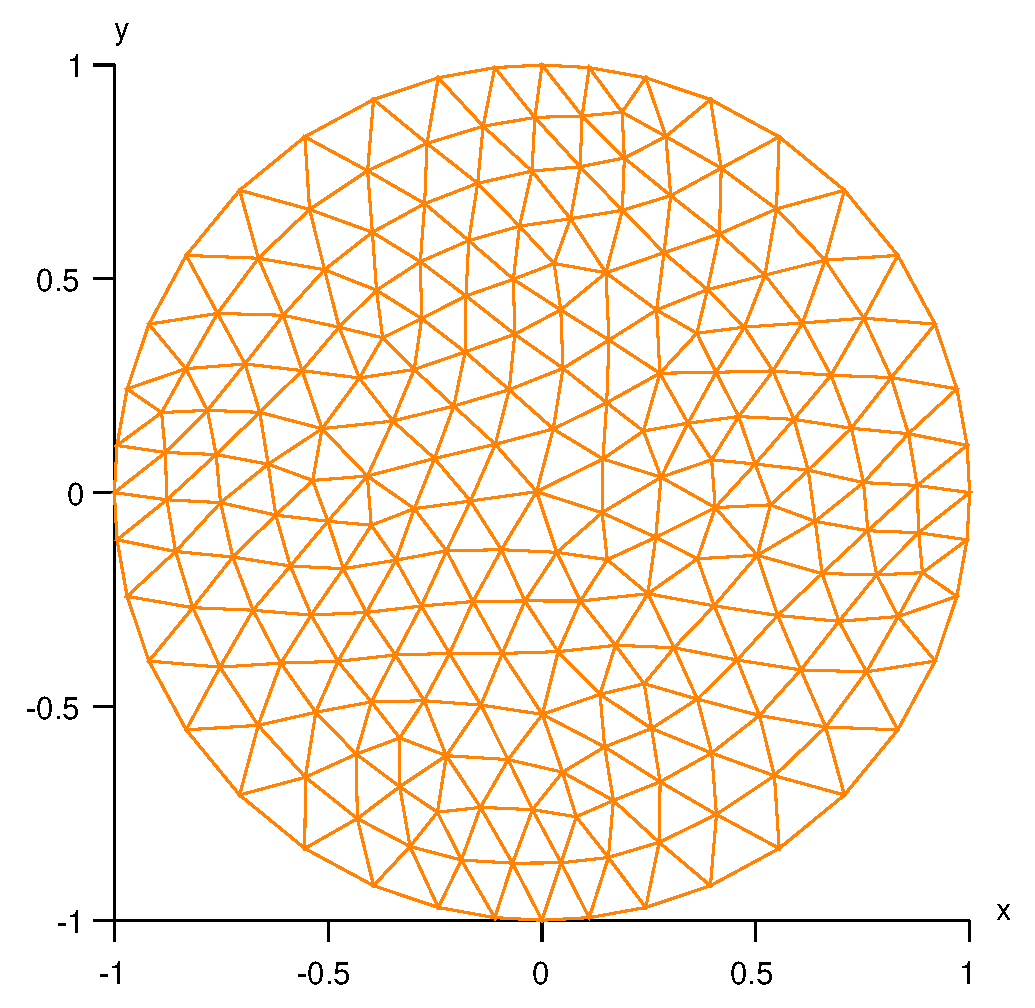
\includegraphics[width=75mm]{disk-with-tri}
 \caption{Circle built from patches, interior of disk meshed progressively}
 \label{\numb section 3.\numb fig 1}
\end{figure}

\begin{Verbatim}[commandchars=\\\{\},formatcom=\small\tt,frame=single,
   label=parag-\ref{\numb section 3.\numb parag 1}.cpp,rulecolor=\color{coment},
   baselinestretch=0.94,framesep=2mm                                            ]
   \verm{Manifold} \azul{RR2} ( \verm{tag}::Euclid, \verm{tag}::of_dim, 2 );
   \verm{Function} \azul{xy} = RR2.build_coordinate_system ( \verm{tag}::Lagrange, \verm{tag}::of_degree, 1 );
   \verm{Function} \azul{x} = xy[0],  \azul{y} = xy[1];
   
   \verm{Manifold} \azul{circle_manif} = RR2.implicit ( x*x + y*y == 1. );
   
   \verm{Cell} \azul{N} ( \verm{tag}::vertex );  x(N) =  0.;   y(N) =  1.;
   \verm{Cell} \azul{W} ( \verm{tag}::vertex );  x(W) = -1.;   y(W) =  0.;
   \verm{Cell} \azul{S} ( \verm{tag}::vertex );  x(S) =  0.;   y(S) = -1.;
   \verm{Cell} \azul{E} ( \verm{tag}::vertex );  x(E) =  1.;   y(E) =  0.;
   \verm{Mesh} \azul{NW} ( \verm{tag}::segment, N.reverse(), W, \verm{tag}::divided_in, 10 );
   \verm{Mesh} \azul{WS} ( \verm{tag}::segment, W.reverse(), S, \verm{tag}::divided_in, 10 );
   \verm{Mesh} \azul{SE} ( \verm{tag}::segment, S.reverse(), E, \verm{tag}::divided_in, 10 );
   \verm{Mesh} \azul{EN} ( \verm{tag}::segment, E.reverse(), N, \verm{tag}::divided_in, 10 );
   \verm{Mesh} \azul{circle} ( \verm{tag}::join, NW, WS, SE, EN );
   
   RR2.set_as_working_manifold();
   \verm{Mesh} \azul{disk} ( \verm{tag}::progressive, \verm{tag}::boundary, circle, \verm{tag}::desired_length, 0.157 );
\end{Verbatim}

We provide the desired length of the segments of the future mesh as an argument to the
constructor.
Of course the length of the segments inside the mesh will vary slightly.
We must take care to give as boundary a curve with segments of length approximatively equal
to the desired length (paragraph \ref{\numb section 3.\numb parag 16} discusses
this requirement).

Paragraph \ref{\numb section 11.\numb parag 3} gives more details about {\small\tt \verm{tag}}s.


          %----------------%
\section{~~Meshing a circle}\label{\numb section 3.\numb parag 2}
          %----------------%

Instead of building the circle by joining four (curved) segments, we can mesh directly
the circle manifold, then mesh the disk :

\begin{Verbatim}[commandchars=\\\{\},formatcom=\small\tt,frame=single,
   label=parag-\ref{\numb section 3.\numb parag 2}.cpp,rulecolor=\color{coment},
   baselinestretch=0.94,framesep=2mm                                            ]
   \verm{Manifold} \azul{RR2} ( \verm{tag}::Euclid, \verm{tag}::of_dim, 2 );
   \verm{Function} \azul{xy} = RR2.build_coordinate_system ( \verm{tag}::Lagrange, \verm{tag}::of_degree, 1 );
   \verm{Function} \azul{x} = xy[0],  \azul{y} = xy[1];
   
   \verm{Manifold} \azul{circle_manif} = RR2.implicit ( x*x + y*y == 1. );
   \verm{Mesh} \azul{circle} ( \verm{tag}::progressive,
      \verm{tag}::entire_manifold, circle_manif, \verm{tag}::desired_length, 0.2 );
   \cinza{// we can omit the manifold; maniFEM will take the current working manifold :}
   \cinza{// Mesh circle ( tag::progressive, tag::desired_length, 0.2 );}
   
   RR2.set_as_working_manifold();
   \verm{Mesh} \azul{disk} ( \verm{tag}::progressive, \verm{tag}::boundary, circle, \verm{tag}::desired_length, 0.2 );
   disk.draw_ps (\verde{"disk.eps"});
\end{Verbatim}

The code above is quite comfortable for the user; he or she only needs to define
the manifold(s) to be meshed and provide the desired (average) length of segments
in the future mesh.
However, this comfort comes at the price of a significant computational effort.
For building the {\small\tt circle}, {\ManiFEM} must first find a starting point for the process
of progressive mesh generation.
In extreme cases, the algorithm may fail to find a starting point on the given manifold.

The user may choose to be more specific in order to save computation time,
by providing a starting point :

\begin{Verbatim}[commandchars=\\\{\},formatcom=\small\tt,
   baselinestretch=0.94,framesep=2mm                      ]
   \verm{Cell} \azul{A} ( \verm{tag}::vertex );  x(A) = 1.;  y(A) = 0.;
   \verm{Mesh} \azul{circle} ( \verm{tag}::progressive, \verm{tag}::start_at, A, \verm{tag}::desired_length, 0.2 );
\end{Verbatim}

Also, {\maniFEM} must infer the right orientation of the {\small\tt circle}
as explained in paragraphs \ref{\numb section 3.\numb parag 10} and
\ref{\numb section 3.\numb parag 13}.
Choosing the other orientation would result in an endless process of meshing the exterior of
the disk.
The process of choosing the right orientation implies some computational effort.
The user can make things easier for {\maniFEM} either by attaching an orientation
to the manifold {\small\tt circle\_\,manif} [this feature is not implemented yet] or
by providing the initial direction as shown in paragraph \ref{\numb section 3.\numb parag 12}.


          %----------------%
\section{~~Inner boundaries}\label{\numb section 3.\numb parag 3}
          %----------------%

Inner boundaries must have the reverse orientation :

\begin{Verbatim}[commandchars=\\\{\},formatcom=\small\tt,frame=single,
   label=parag-\ref{\numb section 3.\numb parag 3}.cpp,rulecolor=\color{coment},
   baselinestretch=0.94,framesep=2mm                                            ]
   \verm{Manifold} \azul{circle} = RR2.implicit ( x*x + y*y == 1. );
   \verm{Mesh} \azul{outer} ( \verm{tag}::progressive, \verm{tag}::desired_length, 0.1 );
   \verm{Manifold} \azul{ellipse} = RR2.implicit ( x*x + (y-0.37)*(y-0.37) + 0.3*x*y == 0.25 );
   \verm{Mesh} \azul{inner} ( \verm{tag}::progressive, \verm{tag}::desired_length, 0.1 );
   \verm{Mesh} \azul{bdry} ( \verm{tag}::join, outer, inner.reverse() );
   RR2.set_as_working_manifold();
   \verm{Mesh} \azul{disk} ( \verm{tag}::progressive, \verm{tag}::boundary, bdry, \verm{tag}::desired_length, 0.1 );
\end{Verbatim}

\begin{figure}[ht] \centering
 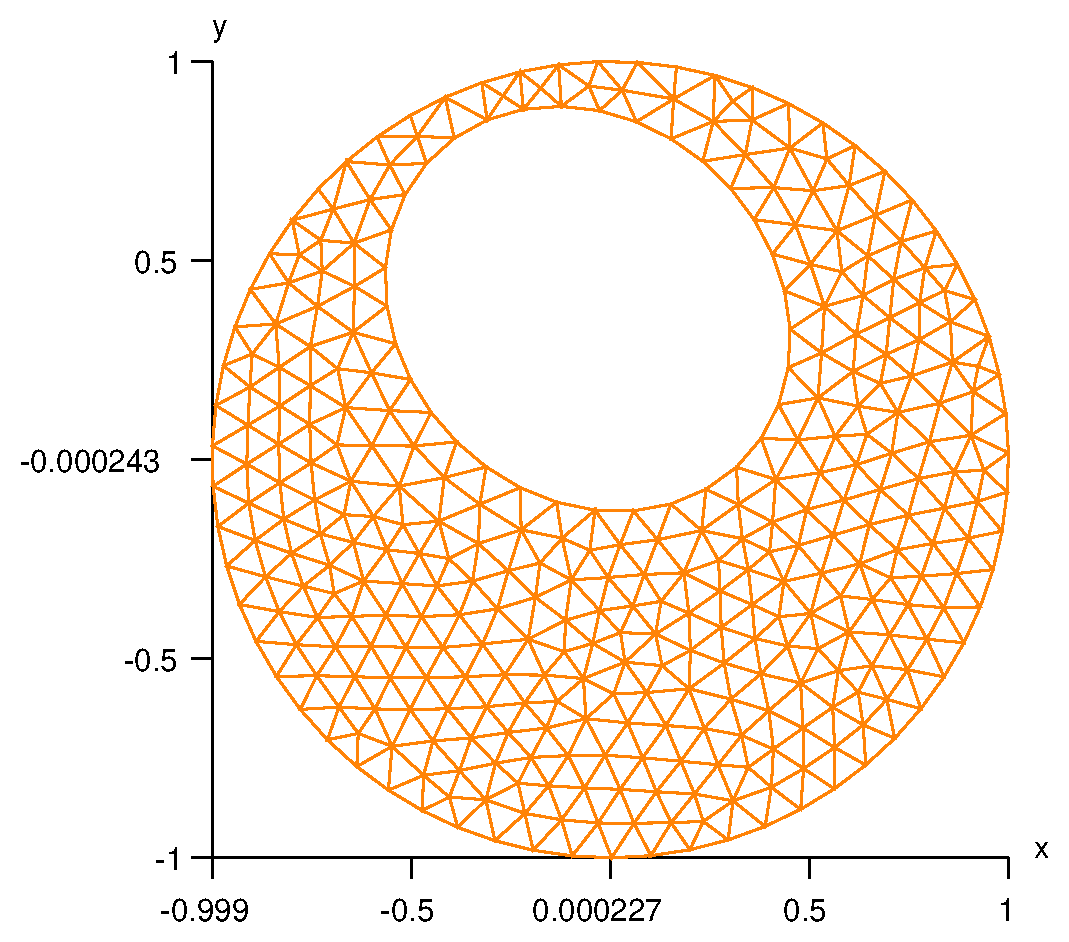
\includegraphics[width=80mm]{disk-with-hole}
  \caption{Disk with a hole}
  \label{\numb section 3.\numb fig 2}
\end{figure}

Paragraphs \ref{\numb section 1.\numb parag 2} and \ref{\numb section 1.\numb parag 3} explain
the relation between the orientation of a mesh and the orientation of its boundary.

Paragraphs \ref{\numb section 3.\numb parag 10} and \ref{\numb section 3.\numb parag 13}
explain how {\maniFEM} chooses the orientation of closed curves.


          %--------------------------------%
\section{~~Meshing a three-dimensional loop}\label{\numb section 3.\numb parag 4}
          %--------------------------------%

We may apply the same {\small\tt progressive} algorithm for meshing the circle in
$ \mathbb{R}^3 $ introduced in paragraph \ref{\numb section 2.\numb parag 12} :

\begin{Verbatim}[commandchars=\\\{\},formatcom=\small\tt,frame=single,
   label=parag-\ref{\numb section 3.\numb parag 4}.cpp,rulecolor=\color{coment},
   baselinestretch=0.94,framesep=2mm                                            ]
   \verm{Manifold} \azul{RR3} ( \verm{tag}::Euclid, \verm{tag}::of_dim, 3 );
   \verm{Function} \azul{xyz} = RR3.build_coordinate_system ( \verm{tag}::Lagrange, \verm{tag}::of_degree, 1 );
   \verm{Function} \azul{x} = xyz[0],  \azul{y} = xyz[1],  \azul{z} = xyz[2];
   \verm{Manifold} \azul{circle_manif} = RR3.implicit ( x*x + y*y == 1., x*y == 4.*z );
   
   \verm{Mesh} \azul{circle}
      ( \verm{tag}::progressive, \verm{tag}::desired_length, 0.1, \verm{tag}::random_orientation );
\end{Verbatim}

Unlike for the {\small\tt circle} in paragraph \ref{\numb section 3.\numb parag 2},
there is no way to choose between the two possible orientations of this {\small\tt circle}.
No one is more ``correct'' than the other.
This is why {\maniFEM} requires a supplementary argument
{\small\tt \verm{tag}::random\_\,orientation}
for the {\small\tt \verm{Mesh}} constructor.
In other cases (e.g.\ for closed curves in $ \mathbb{R}^2 $) this supplementary argument
is not mandatory; however, even then the user may choose to provide the argument
{\small\tt \verm{tag}::random\_\,orientation}, thus sparing the computer from the burden of
finding the right orientation.
Paragraphs \ref{\numb section 3.\numb parag 10} and \ref{\numb section 3.\numb parag 13}
give more details.

On the other hand, if the orientation matters for you, you can either attach an orientation
to the manifold {\small\tt circle\_\,manif} [this feature is not implemented yet]
or provide a starting point and an initial direction as shown in paragraph
\ref{\numb section 3.\numb parag 12}.


          %----------------------------%
\section{~~Starting and stopping points}\label{\numb section 3.\numb parag 5}
          %----------------------------%

In paragraphs \ref{\numb section 3.\numb parag 2} and \ref{\numb section 3.\numb parag 4}
we have meshed the entire closed curve {\small\tt circle}.
If we only want a piece of a curve, we must specify two points, one for starting and
the other one for stopping.

Looking at the example in paragraph \ref{\numb section 2.\numb parag 14}, let us define a
spiral with a slightly different look and switch to progressive mesh generation.

\begin{Verbatim}[commandchars=\\\{\},formatcom=\small\tt,frame=single,
   label=parag-\ref{\numb section 3.\numb parag 5}.cpp,rulecolor=\color{coment},
   baselinestretch=0.94,framesep=2mm                                            ]
   \verm{Manifold} \azul{RR2} ( \verm{tag}::Euclid, \verm{tag}::of_dim, 2 );
   \verm{Function} \azul{xy} = RR2.build_coordinate_system ( \verm{tag}::Lagrange, \verm{tag}::of_degree, 1 );
   \verm{Function} \azul{x} = xy[0],  \azul{y} = xy[1];
   \verm{Function} \azul{r} = \verm{power} ( x*x + y*y, 0.25 );
   const double \azul{pi} = 3.14159;
   
   RR2.implicit ( x*\verm{sin}(r) == y*\verm{cos}(r) );
   \cinza{// we don't need to give a name to the implicit manifold}
   \cinza{// the Manifold constructor sets the manifold it builds as working manifold}
   \cinza{// after that, many methods use this working manifold by default}
   
   \verm{Cell} \azul{A} ( \verm{tag}::vertex );  x(A) =    pi*pi;   y(A) =  0.;
   \verm{Cell} \azul{B} ( \verm{tag}::vertex );  x(B) = 81*pi*pi;   y(B) =  0.;
   \verm{Mesh} \azul{spiral} ( \verm{tag}::progressive, \verm{tag}::start_at, A,
                 \verm{tag}::stop_at, B, \verm{tag}::desired_length, 1. );
\end{Verbatim}

\begin{figure} \centering
  \psfrag{A}{\tt\textcolor{textindraw}{A}}
  \psfrag{B}{\tt\textcolor{textindraw}{B}}
 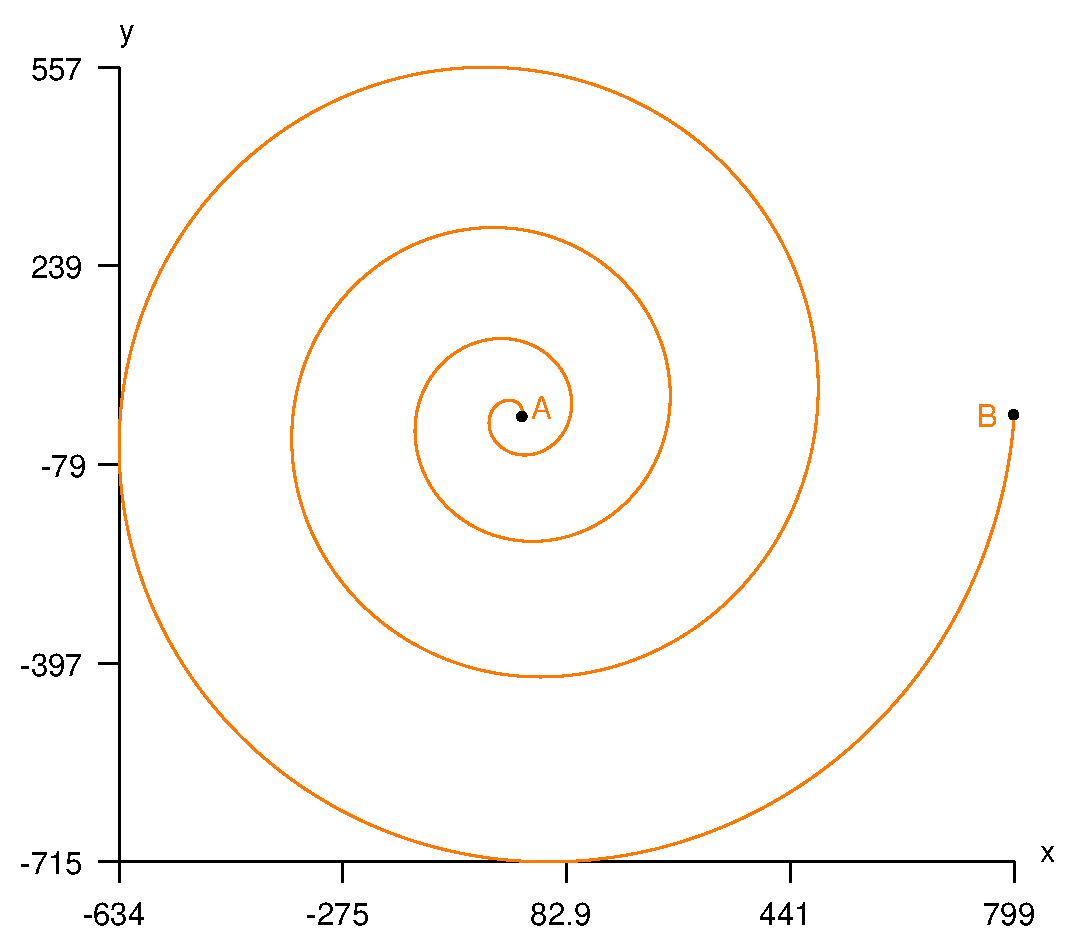
\includegraphics[width=75mm]{spiral-prog}
  \caption{Spiral, meshed progressively}
 \label{\numb section 3.\numb fig 3}
\end{figure}

Figure \ref{\numb section 3.\numb fig 3} shows the resulting mesh.

Unlike in paragraph \ref{\numb section 2.\numb parag 14}, we define the spiral through
an implicit equation.
Had we chosen the (natural) definition {\small\tt r = \verm{power} ( x*x + y*y, 0.5 )},
the very same spiral as in paragraph \ref{\numb section 2.\numb parag 14} would have been
obtained.
For aesthetic reasons, we have chosen a different definition of {\small\tt r}, thus obtaining
a different spacing between the arcs of the spiral.

Another noteworthy difference from paragraph \ref{\numb section 2.\numb parag 14} is that
vertices are distributed uniformly along the spiral (with respect to the distance
in the surrounding space $ \mathbb{R}^2 $).
The segments are too small to be seen in the figure.

Note that there are two ways to go along the spiral starting from {\small\tt A}.
One of them will eventually stumble upon the stopping point {\small\tt B} while
the other one will never meet {\small\tt B}.
{\ManiFEM} has no means to guess which way it should start building the mesh,
so it performs a preliminary search in both directions.
The one that first meets {\small\tt B} wins and the mesh is subsequently built along
the winning direction.

Thus, if we want to mesh an arc of a circle, we can use a sequence of statements like

\begin{Verbatim}[commandchars=\\\{\},formatcom=\small\tt,
   baselinestretch=0.94,framesep=2mm                      ]

   RR2.implicit ( (x-x0)*(x-x0) + (y-y0)*(y-y0) == radius * radius );
   \verm{Cell} \azul{A} ( \verm{tag}::vertex );  \cinza{// set x(A) and y(A)}
   \verm{Cell} \azul{B} ( \verm{tag}::vertex );  \cinza{// set x(B) and y(B)}
   \verm{Mesh} \azul{arc_of_circle} ( \verm{tag}::progressive, \verm{tag}::start_at, A,
                        \verm{tag}::stop_at, B, \verm{tag}::desired_length, some_value );
\end{Verbatim}

However, if we choose {\small\tt A} and {\small\tt B} diametrally opposed, {\maniFEM} will
mesh unpredictably one half of the circle or the other.

Paragraph \ref{\numb section 3.\numb parag 12} shows how we can specify the direction we
want to follow starting from a given point, thus avoiding ambiguities and also saving
computational time.

Of course we must be careful to choose starting and stopping points belonging to the manifold
(or to {\small\tt project} them explicitly -- for this we should have given a name to the
implicit manifold) otherwise the meshing algorithm will either fail to start or will spin
for ever on the circle or spiral, hopelessly searching for {\small\tt B}.


          %-------------------------%
\section{~~Meshing a compact surface}\label{\numb section 3.\numb parag 6}
          %-------------------------%

Recall that in this manual we use the term ``manifold'' to mean a manifold without boundary.
So, the term ``compact surface'' should be understood as ``compact surface without boundary''
like the sphere or the torus.

Just like for the {\small\tt circle} in paragraphs \ref{\numb section 3.\numb parag 2} and
\ref{\numb section 3.\numb parag 4}, if we want to mesh a compact surface entirely
the mesh will have no boundary so we only need to provide the desired (average) length
of segments.
Code below builds a mesh on the sphere.

\begin{Verbatim}[commandchars=\\\{\},formatcom=\small\tt,frame=single,
   label=parag-\ref{\numb section 3.\numb parag 6}.cpp,rulecolor=\color{coment},
   baselinestretch=0.94,framesep=2mm                                            ]
   \verm{Manifold} \azul{RR3} ( \verm{tag}::Euclid, \verm{tag}::of_dim, 3 );
   \verm{Function} \azul{xyz} = RR3.build_coordinate_system ( \verm{tag}::Lagrange, \verm{tag}::of_degree, 1 );
   \verm{Function} \azul{x} = xyz[0],  \azul{y} = xyz[1],  \azul{z} = xyz[2];
   \verm{Manifold} \azul{sphere_manif} = RR3.implicit ( x*x + y*y + z*z == 1. );
   \verm{Mesh} \azul{sphere} ( \verm{tag}::progressive, \verm{tag}::desired_length, 0.1 );
\end{Verbatim}

Again, a significant computational effort is made for finding a starting point
for the meshing process.
We can alleviate this burden simply by providing a starting point on the sphere :

\begin{Verbatim}[commandchars=\\\{\},formatcom=\small\tt,
   baselinestretch=0.94,framesep=2mm                     ]
   \verm{Cell} \azul{A} ( \verm{tag}::vertex );  x(A) = 1.;  y(A) = 0.;  z(A) = 0.;
   \verm{Mesh} \azul{sphere} ( \verm{tag}::progressive, \verm{tag}::start_at, A, \verm{tag}::desired_length, 0.1 );
\end{Verbatim}

Also, some computational effort is made for choosing the right orientation of the sphere;
paragraphs \ref{\numb section 3.\numb parag 10} and \ref{\numb section 3.\numb parag 13}
give more details.


          %--------------------------%
\section{~~A more complicated surface}\label{\numb section 3.\numb parag 7}
          %--------------------------%

Here is an example of a compact surface given by a more complicated implicit equation.
It can be vaguely described as a convolution between two tori.

\begin{Verbatim}[commandchars=\\\{\},formatcom=\small\tt,frame=single,
   label=parag-\ref{\numb section 3.\numb parag 7}.cpp,rulecolor=\color{coment},
   baselinestretch=0.94,framesep=2mm                                            ]
   \verm{Manifold} \azul{RR3} ( \verm{tag}::Euclid, \verm{tag}::of_dim, 3 );
   \verm{Function} \azul{xyz} = RR3.build_coordinate_system ( \verm{tag}::Lagrange, \verm{tag}::of_degree, 1 );
   \verm{Function} \azul{x} = xyz[0],  \azul{y} = xyz[1],  \azul{z} = xyz[2];

   \verm{Function} \azul{f1} = x*x + y*y + 0.1;  \cinza{// we add 0.1 to avoid singularities}
   \verm{Function} \azul{f2} = 1. - \verm{power} ( f1, -0.5 );
   \verm{Function} \azul{d1} = z*z + f1 * f2 * f2;  \cinza{// squared distance to a circle in the xy plane}
   \verm{Function} \azul{f3} = (x-0.4)*(x-0.4) + z*z + 0.1;  \cinza{// we add 0.1 to avoid singularities}
   \verm{Function} \azul{f4} = 1. - \verm{power} ( f3, -0.5 );
   \verm{Function} \azul{d2} = y*y + f3 * f4 *f4;  \cinza{// squared distance to a circle in the xz plane}
   \verm{Manifold} \azul{tori_manif} = RR3.implicit
      ( \verm{smooth_min} ( d1, d2, \verm{tag}::threshold, 0.2 ) == 0.15 );

   \verm{Mesh} \azul{tori} ( \verm{tag}::progressive, \verm{tag}::desired_length, 0.09 );
\end{Verbatim}

\begin{figure}[ht] \centering
 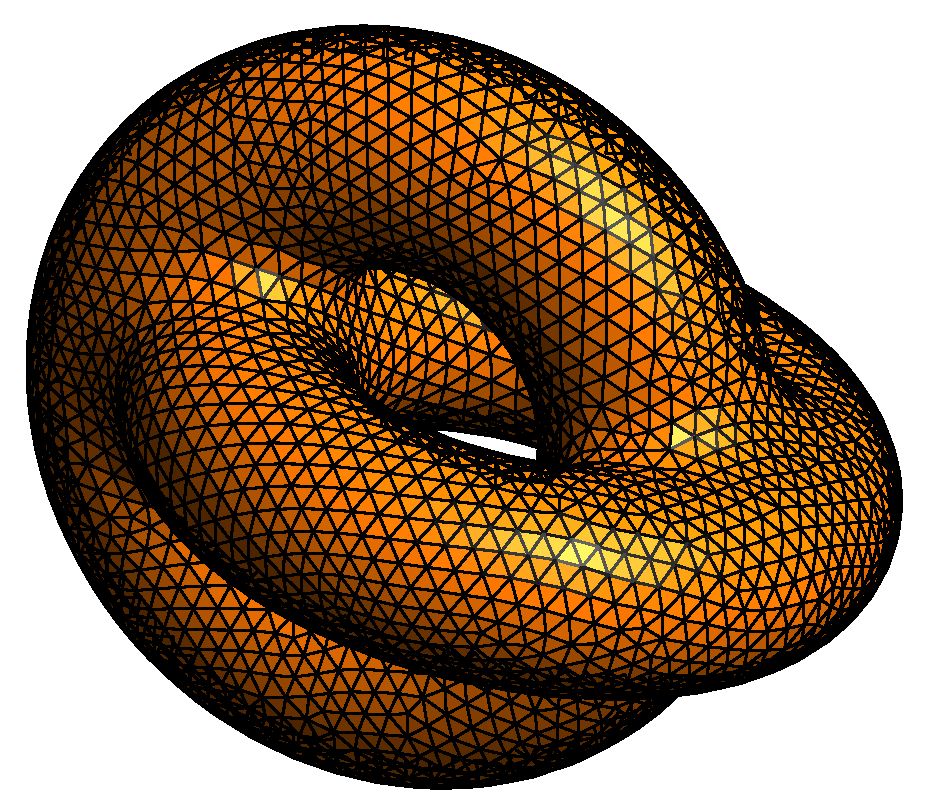
\includegraphics[width=80mm]{two-tori}
  \caption{Convolution between two tori}
\end{figure}

Function {\small\tt \verm{smooth\_\,min}} gives a smooth approximation of the minimum between
two or more {\small\tt \verm{Function}} objects.
It is equal to the true minimum if the difference between the two values is higher, in
absolute value, than the provided threshold.
When the difference is smaller than the threshold, it gives a $ C^1 $ interpolation between
the two values.

If we want sharp edges, we must build the edges first as explained in paragraphs
\ref{\numb section 3.\numb parag 18} and \ref{\numb section 3.\numb parag 19}.

Comments at the end of paragraph \ref{\numb section 3.\numb parag 6} apply here, too :
{\maniFEM} must find a starting point and the right orientation.


\section{~~\cinza{[empty]}}\label{\numb section 3.\numb parag 8}


          %------------------%
\section{~~A bumpy hemisphere}\label{\numb section 3.\numb parag 9}
          %------------------%

We now look again at the surface in paragraph \ref{\numb section 2.\numb parag 13}
and build it progressively, using fewer lines of code.

\begin{Verbatim}[commandchars=\\\{\},formatcom=\small\tt,
   baselinestretch=0.94,framesep=2mm                      ]
   \verm{Manifold} \azul{nut} = RR3.implicit ( x*x + y*y + z*z + 1.5*x*y*z == 1. );
   \verm{Manifold} \azul{base} = nut.implicit ( x*x + 3.*z == 0. );
   \verm{Mesh} \azul{circle}  \cinza{// 'base' is used by default as working manifold}
      ( \verm{tag}::progressive, \verm{tag}::desired_length, 0.1, \verm{tag}::random_orientation );
   
   nut.set_as_working_manifold();
   \verm{Mesh} \azul{bumpy}  \cinza{// 'nut' is used as working manifold}
      ( \verm{tag}::progressive, \verm{tag}::boundary, circle, \verm{tag}::desired_length, 0.1 );
\end{Verbatim}

In this example, the issue of the orientation can be really tricky.
An orientation of the {\small\tt circle} is chosen at random.
Also, {\maniFEM} will randomly choose to mesh the upper or the lower hemisphere.
Paragraphs \ref{\numb section 3.\numb parag 10}, \ref{\numb section 3.\numb parag 13} and
\ref{\numb section 3.\numb parag 14} give more details.


          %-----------------------------%
\section{~~How the orientation is chosen}\label{\numb section 3.\numb parag 10}
          %-----------------------------%

In \maniFEM, cells and meshes are oriented (paragraphs \ref{\numb section 1.\numb parag 2}
and \ref{\numb section 9.\numb parag 5} provide details).
For building a mesh progressively, {\maniFEM} needs to know which orientation we want.

Manifolds may be oriented or not.
Euclidian manifolds (that is, the space $ \mathbb{R}^n $) have an intrinsic orientation,
given by the natural order of the $n$ coordinates.
Parametric manifolds inherit the intrinsic orientation from the space of parameters.
Implicit manifolds, however, have no intrinsic orientation.
We can specify an orientation of a manifold by attaching an outer form to it
(this feature is not implemented yet); otherwise, it will be considered not oriented.

In the example in paragraph \ref{\numb section 3.\numb parag 1}, the boundary {\small\tt circle}
is oriented according to the four segments composing it, {\small\tt NW}, {\small\tt WS},
{\small\tt SE} and {\small\tt EN}.
\ {\ManiFEM} uses the intrinsic orientation of the surrounding space {\small\tt RR2} in order
to determine the desired orientation of the mesh {\small\tt disk}.
The orientation of the boundary {\small\tt circle} is important;
together with the intrinsic orientation of the surrounding space,
it determines on which side of the circle the mesh will be propagated.
Had we built the segments {\small\tt NW}, {\small\tt WS}, {\small\tt SE} and {\small\tt EN} in the
opposite direction (that is, {\small\tt WN}, {\small\tt SW}, {\small\tt ES} and {\small\tt NE})
the program would have tried to mesh the exterior of the disk, never stopping.

Compact manifolds of co-dimension one (closed curves in $ \mathbb{R}^2 $,
compact surfaces in $ \mathbb{R}^3 $) are an exception among implicit manifolds.
Recall that in this manual we use the term ``manifold'' to mean a manifold without boundary.
There is a ``privileged'' orientation of a compact manifold of co-dimension one,
which is compatible with the intrinsic orientation of the surrounding space.
We call this orientation {\small\tt inherent}; paragraph \ref{\numb section 3.\numb parag 13}
discusses this topic.

Open curves (like the spiral in paragraps \ref{\numb section 3.\numb parag 5} and
\ref{\numb section 3.\numb parag 12}) have no privileged orientation.
If we don't specify an orientation, these manifolds are considered not oriented.
If we don't specify a starting direction, {\maniFEM} will perform a preliminary search
in both directions and choose the one that first meets the stopping point.

Closed curves in $ \mathbb{R}^3 $ like the {\small\tt circle} in paragraphs
\ref{\numb section 3.\numb parag 4} and \ref{\numb section 3.\numb parag 9}
have no privileged orientation either.
There is no way to decide which of its two possible orientations
should be chosen; no one is more ``correct'' than the other.
This is why {\maniFEM} will reject a tentative to define {\small\tt circle} without
{\small\tt \verm{tag}::random\_\,orientation} as last argument to the {\small\tt \verm{Mesh}} constructor.
A statement like {\small\tt \verm{Mesh}} {\small\tt circle} {\small\tt (}
{\small\tt \verm{tag}::progressive,} {\small\tt\verm{tag}::desired\_\,length,}
{\small\tt some\_\,value )}
will produce a run-time error if the current working manifold has dimension 1 and
the geometric dimension (that is, the number of coordinates) is 3.

The options given to the constructor of {\small\tt \verm{Mesh} bumpy} in paragraph
\ref{\numb section 3.\numb parag 9} are discussed in paragraph
\ref{\numb section 3.\numb parag 14}.


\section{~~\cinza{[empty]}}\label{\numb section 3.\numb parag 11}


          %------------------------%
\section{~~Specifying the direction}\label{\numb section 3.\numb parag 12}
          %------------------------%

For one-dimensional manifolds, we can specify, along with the starting point,
a starting direction, thus saving some computational time.
The code producing the spiral in paragraph \ref{\numb section 3.\numb parag 5}
can be changed as below.

\begin{Verbatim}[commandchars=\\\{\},formatcom=\small\tt,frame=single,
   label=parag-\ref{\numb section 3.\numb parag 12}.cpp,rulecolor=\color{coment},
   baselinestretch=0.94,framesep=2mm                                            ]
   \verm{Cell} \azul{A} ( \verm{tag}::vertex );  x(A) =    pi*pi;   y(A) =  0.;
   \verm{Cell} \azul{B} ( \verm{tag}::vertex );  x(B) = 81*pi*pi;   y(B) =  0.;
   std::vector < double > \azul{direc} = \{ 0., 1. \};
   \verm{Mesh} \azul{spiral} ( \verm{tag}::progressive, \verm{tag}::start_at, A, \verm{tag}::towards, direc,
                 \verm{tag}::stop_at, B, \verm{tag}::desired_length, 1.                 );
\end{Verbatim}

Note that the vector {\small\tt direc} is associated to the point {\small\tt A}.

Recall that open curves have no ``default'' (or ``inherent'') orientation.
{\ManiFEM} uses the vector {\small\tt direc} as an indication about where to go.

It is the user's responsibility to ensure that, going in the specified direction,
the algorithm will eventually meet the stopping point {\small\tt B}.
Otherwise, we may end up spinning endlessly along the spiral.

We could specify in a similar fashion the orientation of {\small\tt circle} in paragraph
\ref{\numb section 3.\numb parag 2}, thus saving some computational time :

\begin{Verbatim}[commandchars=\\\{\},formatcom=\small\tt,
   baselinestretch=0.94,framesep=2mm                                            ]
   \verm{Cell} \azul{A} ( \verm{tag}::vertex );  x(A) = 1.;  y(A) = 0.;
   \verm{Mesh} \azul{circle} ( \verm{tag}::progressive, \verm{tag}::start_at, A,
                 \verm{tag}::towards, \{ 0., 1. \}, \verm{tag}::desired_length, 0.2 );
\end{Verbatim}

If, in the above, we choose the opposite {\small\tt direc}tion,
{\maniFEM} will later try to mesh the exterior of the disk.

The same technique can be used for building the {\small\tt circle} in paragraph
\ref{\numb section 3.\numb parag 4}, thus avoiding \maniFEM's random choice of the orientation :

\begin{Verbatim}[commandchars=\\\{\},formatcom=\small\tt,
   baselinestretch=0.94,framesep=2mm                     ]
   \verm{Cell} \azul{S} ( \verm{tag}::vertex );  x(S) =  0.;   y(S) = -1.;  z(S) = 0.;
   \verm{Manifold} \azul{circle_manif} = RR3.implicit ( x*x + y*y == 1., x*y == 4.*z );
   \verm{Mesh} \azul{circle} ( \verm{tag}::progressive, \verm{tag}::start_at, S,
                 \verm{tag}::towards, \{ 1., 0., 0. \}, \verm{tag}::desired_length, 0.2 );
\end{Verbatim}

This also applies to the example in paragraph \ref{\numb section 3.\numb parag 9}.
However, there the topologic considerations are more complex, so we delegate this
discussion to paragraph \ref{\numb section 3.\numb parag 14}.


          %---------------------------------------%
\section{~~The intrinsic and inherent orientations}\label{\numb section 3.\numb parag 13}
          %---------------------------------------%

Euclidian manifolds have an intrinsic orientation given by the natural order of the
coordinates.
{\ManiFEM} will always use this orientation when the working manifold is Euclidian.
We can enforce the requirement of using the intrinsic orientation by providing a
{\small\tt \verm{tag}::intrinsinc\_\,orien\-tation} as argument to the {\small\tt \verm{Mesh}} constructor.
However, this argument is not necessary; {\maniFEM} will consider it by default.
This happens for the {\small\tt disk} in paragraphs \ref{\numb section 3.\numb parag 1} and
\ref{\numb section 3.\numb parag 2}, for the diamond in
paragraph \ref{\numb section 3.\numb parag 17} and for the annulus in paragraphs
\ref{\numb section 3.\numb parag 3}, \ref{\numb section 3.\numb parag 22}
and \ref{\numb section 3.\numb parag 24}.

Compact manifolds of co-dimension one (closed curves in $ \mathbb{R}^2 $,
compact surfaces in $ \mathbb{R}^3 $) have a privileged orientation,
compatible with the intrinsic orientation of the surrounding space;
we call this orientation ``inherent''.
{\ManiFEM} will choose it in some situations, unless we provide a
{\small\tt \verm{tag}::random\_\,orientation} as argument to the {\small\tt \verm{Mesh}} constructor.
We can enforce the requirement of finding the inherent orientation by providing a
{\small\tt \verm{tag}::inherent\_\,orientation} as argument to the {\small\tt \verm{Mesh}} constructor;
however, {\maniFEM} will consider this argument by default when we provide no stopping
point (for one-dimensional meshes) or we provide no boundary (for two-dimensional meshes).
In these cases, {\maniFEM} will assume that the manifold is compact and, if it has
co-dimension one, the inherent orientation will be used.
This happens for the {\small\tt circle} in paragraph \ref{\numb section 3.\numb parag 2},
for the {\small\tt sphere} in paragraph \ref{\numb section 3.\numb parag 6} and for the
{\small\tt tori} in paragraph \ref{\numb section 3.\numb parag 7}.

If we do provide a stopping point, or a boundary, {\maniFEM} has no means to know in
advance whether the manifold
is compact or not, so it will not try to find the inherent orientation.
This happens for the {\small\tt spiral} and for the {\small\tt arc\_\,of\_\,circle} in paragraph
\ref{\numb section 3.\numb parag 5}, for the {\small\tt bumpy} hemisphere in paragraph
\ref{\numb section 3.\numb parag 9}, for the {\small\tt piece\_\,of\_\,cyl} and
{\small\tt piece\_\,of\_\,sph} in paragraphs \ref{\numb section 3.\numb parag 18} and
\ref{\numb section 3.\numb parag 19} and others.
In these situations, we may require specifically the inherent orientation
by providing the {\small\tt \verm{tag}::inherent\_\,orientation} as last argument to the
{\small\tt \verm{Mesh}} constructor.
Do not misuse this option; if you ask {\maniFEM} to find the inherent orientation of an open
curve or of a non-compact surface, it will not complain but will hopelessly try to mesh
the entire manifold, never stopping.
For instance, in paragraph \ref{\numb section 3.\numb parag 5} it makes sense to enforce the
{\small\tt inherent\_\,orientation} for the {\small\tt arc\_\,of\_\,circle} but not for the
{\small\tt spiral}.
Also, in paragraphs \ref{\numb section 3.\numb parag 18} and
\ref{\numb section 3.\numb parag 19} it makes sense to enforce the
{\small\tt inherent\_\,orientation} for the
{\small\tt piece\_\,of\_\,sph} but not for the {\small\tt piece\_\,of\_\,cyl}.

Determining the intrinsic orientation of a Euclidian manifold is computationally
very cheap.
However, determining the inherent orientation of a manifold of co-dimension one is not
a trivial computational process.
{\ManiFEM} is unable to determine this orientation by looking at the equations defining
the manifold; it needs a mesh on the entire manifold.

So, in paragraph \ref{\numb section 3.\numb parag 2} we obtain a correctly oriented mesh
on the disk, with no need to provide any specific information about the orientation of
{\small\tt circle\_\,manif}.
Behind the curtains, {\maniFEM} builds a mesh on {\small\tt circle\_\,manif} with
an initially arbitrary orientation, then checks its consistency
within the surrounding manifold and, if necessary, switches the orientation of the produced mesh.
Then, again, the orientation of the boundary (together with the intrinsic orientation of
the surrounding space {\small\tt RR2}) defines whether the interior or the exterior of the
disk is to be meshed.

A similar process happens for compact surfaces in $ \mathbb{R}^3 $ like those
considered in paragraphs \ref{\numb section 3.\numb parag 6} and
\ref{\numb section 3.\numb parag 7},
except that checking the orientation of a compact surface has a computational cost
considerably higher than for a closed curve in $ \mathbb{R}^2 $.

You can save some computing time if you specify the orientation
yourself, either by providing more information to the {\small\tt \verm{Mesh}} constructor as shown
in paragraph \ref{\numb section 3.\numb parag 15} or by attaching this information to
the manifold itself (this feature is not implemented yet).
% in order to alleviate the computational burden
 
If the orientation is not important for you, you can add to the {\small\tt \verm{Mesh}} constructor
the last argument {\small\tt \verm{tag}::random\_\,orientation} and {\maniFEM} will not waste
computing time to find the inherent orientation.
\vskip 1mm

          %-------------------------------%
\section{~~Revisiting the bumpy hemisphere}\label{\numb section 3.\numb parag 14}
          %-------------------------------%

%The random behaviour in this example is quite dramatic.
Let us have a closer look at the code in paragraph \ref{\numb section 3.\numb parag 9}.
The manifold {\small\tt nut} has a unique orientation consistent with the surrounding
space, just like those in paragraphs \ref{\numb section 3.\numb parag 6} and
\ref{\numb section 3.\numb parag 7}, but the {\small\tt base} within it has not.
This is why, when we build the {\small\tt circle}, we must provide a
{\small\tt \verm{tag}::random\_\,orientation} as a last argument to the {\small\tt \verm{Mesh}} constructor,
or specify the orientation by providing a starting point and a starting direction
as described in paragraph \ref{\numb section 3.\numb parag 12}.

When we build {\small\tt bumpy}, since we are providing a boundary, {\maniFEM} does not treat
the current working manifold {\small\tt nut} as compact, that is, it does not try to determine an
inherent orientation.
It will start the meshing process on an arbitrary side of {\small\tt circle}, thus meshing
unpredictably the upper or the lower {\small\tt bumpy} hemisphere.

If we enforce the orientation by providing a {\small\tt \verm{tag}::inherent\_\,orientation} as a last
argument to the {\small\tt \verm{Mesh}} constructor of {\small\tt bumpy}, then {\maniFEM} will mesh
(behind the curtains) both halves of the sphere; let's call them {\small\tt msh1} and {\small\tt msh2}.
Note that the {\small\tt circle} has already been built, so its orientation is given.
Both {\small\tt msh1} and {\small\tt msh2} have {\small\tt circle} as boundary,
which means that they have mutually incompatible orientations.
They cannot be {\small\tt join}ed.
But the reverse of any of them can be {\small\tt join}ed with the other one, the result being a
mesh on the entire bumpy sphere.
Two choices are possible : either {\small\tt msh1.reverse()} is {\small\tt join}ed with {\small\tt msh2}
or {\small\tt msh1} is {\small\tt join}ed with {\small\tt msh2.reverse()}, resulting in two meshes on
the same compact surface with opposite orientations.
One of these orientations is compatible with the intrinsic orientation of the surrounding space
$ \mathbb{R}^3 $ and is called inherent orientation.
If the first one is correctly oriented, {\small\tt msh2} will be returned;
if the second one is correctly oriented, {\small\tt msh1} will be returned.

Thus, in the code below we will obtain the upper hemisphere.

\begin{Verbatim}[commandchars=\\\{\},formatcom=\small\tt,
   baselinestretch=0.94,framesep=2mm                      ]
   \verm{Cell} \azul{S} ( \verm{tag}::vertex );  x(S) =  0.;  y(S) = -1.;  z(S) =  0.;
   \verm{Mesh} \azul{circle} ( \verm{tag}::progressive, \verm{tag}::start_at, S, \verm{tag}::towards, \{ 1., 0., 0. \},
                 \verm{tag}::desired_length, 0.1                                         );
   nut.set_as_working_manifold();
   \verm{Mesh} \azul{bumpy} ( \verm{tag}::progressive, \verm{tag}::boundary, circle,
                \verm{tag}::desired_length, 0.1, \verm{tag}::inherent_orientation );
\end{Verbatim}

Code below will produce the lower hemisphere.

\begin{Verbatim}[commandchars=\\\{\},formatcom=\small\tt,
   baselinestretch=0.94,framesep=2mm                      ]
   \verm{Cell} \azul{S} ( \verm{tag}::vertex );    x(S) =  0.;  y(S) = -1.;  z(S) =  0.;
   \verm{Mesh} \azul{circle} ( \verm{tag}::progressive, \verm{tag}::start_at, S, \verm{tag}::towards, \{ -1., 0., 0. \},
                 \verm{tag}::desired_length, 0.1                                          );
   nut.set_as_working_manifold();
   \verm{Mesh} \azul{bumpy} ( \verm{tag}::progressive, \verm{tag}::boundary, circle,
                \verm{tag}::desired_length, 0.1, \verm{tag}::inherent_orientation );
\end{Verbatim}

Code below will unpredictably mesh the upper or the lower hemisphere;
in either case, the produced mesh will be oriented upwards because the orientation
of {\small\tt circle} points upwards.
Here, the word ``upwards'' is used in the sense of the right hand rule
(see paragraph \ref{\numb section 1.\numb parag 2}).

\begin{Verbatim}[commandchars=\\\{\},formatcom=\small\tt,
   baselinestretch=0.94,framesep=2mm                     ]
   \verm{Cell} \azul{S} ( \verm{tag}::vertex );    x(S) =  0.;  y(S) = -1.;  z(S) =  0.;
   \verm{Mesh} \azul{circle} ( \verm{tag}::progressive, \verm{tag}::start_at, S, \verm{tag}::towards, \{ 1., 0., 0. \},
                 \verm{tag}::desired_length, 0.1                                         );
   nut.set_as_working_manifold();
   \verm{Mesh} \azul{bumpy} ( \verm{tag}::progressive, \verm{tag}::boundary, circle, \verm{tag}::desired_length, 0.1 );
\end{Verbatim}

Code below will unpredictably mesh the upper or the lower hemisphere;
in either case, the produced mesh will be oriented downwards.

\begin{Verbatim}[commandchars=\\\{\},formatcom=\small\tt,
   baselinestretch=0.94,framesep=2mm                     ]
   \verm{Cell} \azul{S} ( \verm{tag}::vertex );    x(S) =  0.;  y(S) = -1.;  z(S) =  0.;
   \verm{Mesh} \azul{circle} ( \verm{tag}::progressive, \verm{tag}::start_at, S, \verm{tag}::towards, \{ -1., 0., 0. \},
                 \verm{tag}::desired_length, 0.1                                          );
   nut.set_as_working_manifold();
   \verm{Mesh} \azul{bumpy} ( \verm{tag}::progressive, \verm{tag}::boundary, circle, \verm{tag}::desired_length, 0.1 );
\end{Verbatim}

Code below will still mesh unpredictably either the upper or the lower
hemisphere, but only due to the random choice in the orientation of {\small\tt circle}.
The construction of {\small\tt bumpy} is uniquely determined by the orientation of
{\small\tt circle}.

\begin{Verbatim}[commandchars=\\\{\},formatcom=\small\tt,
   baselinestretch=0.94,framesep=2mm                      ]
   \verm{Manifold} \azul{nut} = RR3.implicit ( x*x + y*y + z*z + 1.5*x*y*z == 1. );
   \verm{Manifold} \azul{base} = nut.implicit ( x*x + 3.*z == 0. );
   \verm{Mesh} \azul{circle}
      ( \verm{tag}::progressive, \verm{tag}::desired_length, 0.1, \verm{tag}::random_orientation );
   nut.set_as_working_manifold();
   \verm{Mesh} \azul{bumpy} ( \verm{tag}::progressive, \verm{tag}::boundary, circle,
                \verm{tag}::desired_length, 0.1, \verm{tag}::inherent_orientation );
\end{Verbatim}


          %------------------------%
\section{~~Specifying the direction}\label{\numb section 3.\numb parag 15}
          %------------------------%

In paragraph \ref{\numb section 3.\numb parag 12} we have seen how we can specify the direction
of propagation of the mesh for one-dimensional manifolds.
A similar approach can be taken for two-dimensional meshes.
For instance, code below will mesh the upper half of the ``bumpy hemisphere'' already considered
in paragraphs \ref{\numb section 2.\numb parag 13}, \ref{\numb section 3.\numb parag 9} and
\ref{\numb section 3.\numb parag 14}, oriented upwards.

\begin{Verbatim}[commandchars=\\\{\},formatcom=\small\tt,frame=single,
   label=parag-\ref{\numb section 3.\numb parag 15}.cpp,rulecolor=\color{coment},
   baselinestretch=0.94,framesep=2mm                                            ]
   \verm{Cell} S ( \verm{tag}::vertex );    x(S) =  0.;  y(S) = -1.;  z(S) =  0.;
   std::vector < double > \azul{tau} \{ 1., 0., 0. \};
   \verm{Mesh} circle ( \verm{tag}::progressive, \verm{tag}::start_at, S, \verm{tag}::towards, tau,
                 \verm{tag}::desired_length, 0.1                               );
   nut.set_as_working_manifold();
   std::vector < double > \azul{N} \{ 0., 0., 1. \};
   \verm{Mesh} bumpy ( \verm{tag}::progressive, \verm{tag}::boundary, circle,
                \verm{tag}::start_at, S, \verm{tag}::towards, N,
                \verm{tag}::desired_length, 0.1                 );
\end{Verbatim}

If we define {\small\tt N} as \catcode`<=1\catcode`>=2\catcode`{=12\catcode`}=12<\small\tt {>
<\small\tt 0.,> <\small\tt 0.,> <\small\tt -1.> <\small\tt }>\catcode`<=12\catcode`>=12\catcode`{=1\catcode`}=2, we will obtain
the lower half of the ``sphere'', still oriented upwards.

If we define {\small\tt tau} as \catcode`<=1\catcode`>=2\catcode`{=12\catcode`}=12<\small\tt {>
<\small\tt -1.,> <\small\tt 0.,> <\small\tt 0.> <\small\tt }>\catcode`<=12\catcode`>=12\catcode`{=1\catcode`}=2, we will get a mesh
oriented downwards.


          %---------------------%
\section{~~Geometric limitations}\label{\numb section 3.\numb parag 16}
          %---------------------%

Progressive meshing has its limits.
{\ManiFEM} cannot mesh a manifold whose curvature is too high when compared to the
length of the segments.
The example in paragraph \ref{\numb section 3.\numb parag 7} is ``on the edge'', that is,
if we increase the segment size the meshing process will probably get stuck somewhere.

Also, we should avoid domains whose boundary has components too close to each other,
when compared to the segment size.
In this respect, the example in paragraph \ref{\numb section 3.\numb parag 3} is also
``on the edge''.
In contrast, {\maniFEM} is ``at ease'' when meshing the same domain with other options,
like in paragraphs \ref{\numb section 3.\numb parag 22}, \ref{\numb section 3.\numb parag 23}
or \ref{\numb section 3.\numb parag 24}.

Sharp edges and singularities must be dealt with as described in subsequent paragraphs.

The example in paragraph \ref{\numb section 3.\numb parag 1} is also ``on the edge''
for a different reason.
While {\maniFEM} tries to build a mesh with segments of constant given length,
the length of the segments on the boundary of the disk varies (paragraphs
\ref{\numb section 2.\numb parag 4} and \ref{\numb section 2.\numb parag 5} explain why).
This contradiction puts the algorithm in a difficult position.
If the variation were larger (or sharper) the algorithm might stop with some error message.
In contrast, {\maniFEM} is ``at ease'' when meshing the disk in paragraph
\ref{\numb section 3.\numb parag 2} because there the segments on the boundary have
(approximately) constant length.


          %------------%
\section{~~Sharp angles}\label{\numb section 3.\numb parag 17}
          %------------%

{\ManiFEM} can deal with non-smooth domains.
The user must define separately smooth pieces of the boundary and then join them.

Here is how to mesh the diamond-shaped domain in paragraph \ref{\numb section 2.\numb parag 10}.

\begin{Verbatim}[commandchars=\\\{\},formatcom=\small\tt,frame=single,
   label=parag-\ref{\numb section 3.\numb parag 17}.cpp,rulecolor=\color{coment},
   baselinestretch=0.94,framesep=2mm                                            ]
   \cinza{// we define the arcs NW, WS, SE and EN either as segments, like in}
   RR2.implicit ( x*y + x - y == -1. );
   \verm{Mesh} \azul{NW} ( \verm{tag}::segment, N.reverse(), W, \verm{tag}::divided_in, 12 );
   
   \cinza{// or with tag::progressive like in}
   RR2.implicit ( x*y - x - y ==  1. );
   \verm{Mesh} \azul{WS} ( \verm{tag}::progressive, \verm{tag}::start_at, W, \verm{tag}::stop_at, S,
             \verm{tag}::desired_length, 0.1 );
   \cinza{// ... //}
             
   \verm{Mesh} \azul{bdry} ( \verm{tag}::join, NW, WS, SE, EN );
   RR2.set_as_working_manifold();
   \verm{Mesh} \azul{diamond} ( \verm{tag}::progressive, \verm{tag}::boundary, bdry, \verm{tag}::desired_length, 0.1 );
\end{Verbatim}

%Alternatively, we can provide the pieces of boundary separately :

%\begin{Verbatim}[commandchars=\\\{\},formatcom=\small\tt,
%   baselinestretch=0.94,framesep=2mm                      ]
%   \verm{Mesh} diamond ( \verm{tag}::progressive, \verm{tag}::boundary, NW, WS, SE, EN,
%                  \verm{tag}::desired_length, 1.5 );
%\end{Verbatim}

% In this example we can use either syntax.
% There are other examples where we cannot join the pieces of boundary and so we can only
% use the second version of the constructor, like in paragraph
% \ref{\numb section 3.\numb parag 18} for instance.


          %-----------%
\section{~~Sharp edges}\label{\numb section 3.\numb parag 18}
          %-----------%

We can mesh surfaces with sharp edges, by building individually smooth pieces of surface
and then {\small\tt join}ing them.
The edges must be built first;
thus, some previous knowledge about the geometry of the surface is needed.

\begin{Verbatim}[commandchars=\\\{\},formatcom=\small\tt,frame=single,
   label=parag-\ref{\numb section 3.\numb parag 18}.cpp,rulecolor=\color{coment},
   baselinestretch=0.94,framesep=2mm                                            ]
   \verm{Manifold} \azul{RR3} ( \verm{tag}::Euclid, \verm{tag}::of_dim, 3 );
   \verm{Function} \azul{xyz} = RR3.build_coordinate_system ( \verm{tag}::Lagrange, \verm{tag}::of_degree, 1 );
   \verm{Function} \azul{x} = xyz[0],  \azul{y} = xyz[1],  \azul{z} = xyz[2];

   const double rs = 1.;    \cinza{// radius of the sphere}
   const double rc = 0.45;  \cinza{// radius of the cylinder}
   const double seg_size = 0.1;

   \verm{Manifold} \azul{cylinder} = RR3.implicit ( y*y + (z-0.5)*(z-0.5) == rc*rc );

   cylinder.implicit ( x == 1.5 );  \cinza{// we cut the cylinder on its right side}
   \verm{Cell} \azul{start_1} ( \verm{tag}::vertex );
   x ( start_1 ) = 1.5;  y ( start_1 ) = 0.;  z ( start_1 ) = 0.5 + rc;
   \verm{Mesh} \azul{circle_1} ( \verm{tag}::progressive, \verm{tag}::start_at, start_1,
                   \verm{tag}::towards, \{ 0., 1., 0. \}, \verm{tag}::desired_length, seg_size );

   \cinza{// we cut the cylinder on its left side with a sphere}
   \verm{Manifold} \azul{intersection} = cylinder.implicit ( x*x + y*y + z*z == rs*rs );
   \verm{Cell} \azul{start_2} ( \verm{tag}::vertex );
   x ( start_2 ) = 1.;  y ( start_2 ) = 0.;  z ( start_2 ) = 0.5 - rc;
   intersection.project ( start_2 );
   \verm{Mesh} \azul{circle_2} ( \verm{tag}::progressive, \verm{tag}::start_at, start_2,
                   \verm{tag}::towards, \{ 0., -1., 0. \}, \verm{tag}::desired_length, seg_size );

   \verm{Mesh} \azul{two_circles} ( \verm{tag}::join, circle_1, circle_2.reverse() );
   cylinder.set_as_working_manifold();
   \verm{Mesh} \azul{piece_of_cyl} ( \verm{tag}::progressive, \verm{tag}::boundary, two_circles,
                       \verm{tag}::start_at, start_1, \verm{tag}::towards, \{ -1., 0., 0. \},
                       \verm{tag}::desired_length, seg_size                          );

   RR3.implicit ( x*x + y*y + z*z == rs*rs );
   \verm{Mesh} \azul{piece_of_sph} ( \verm{tag}::progressive, \verm{tag}::boundary, circle_2,
                       \verm{tag}::start_at, start_2, \verm{tag}::towards, \{ 0., 0., -1. \},
                       \verm{tag}::desired_length, seg_size                         );
                       
   \verm{Mesh} \azul{sphere_and_cylinder} ( \verm{tag}::join, piece_of_sph, piece_of_cyl );
\end{Verbatim}

\begin{figure} \centering
 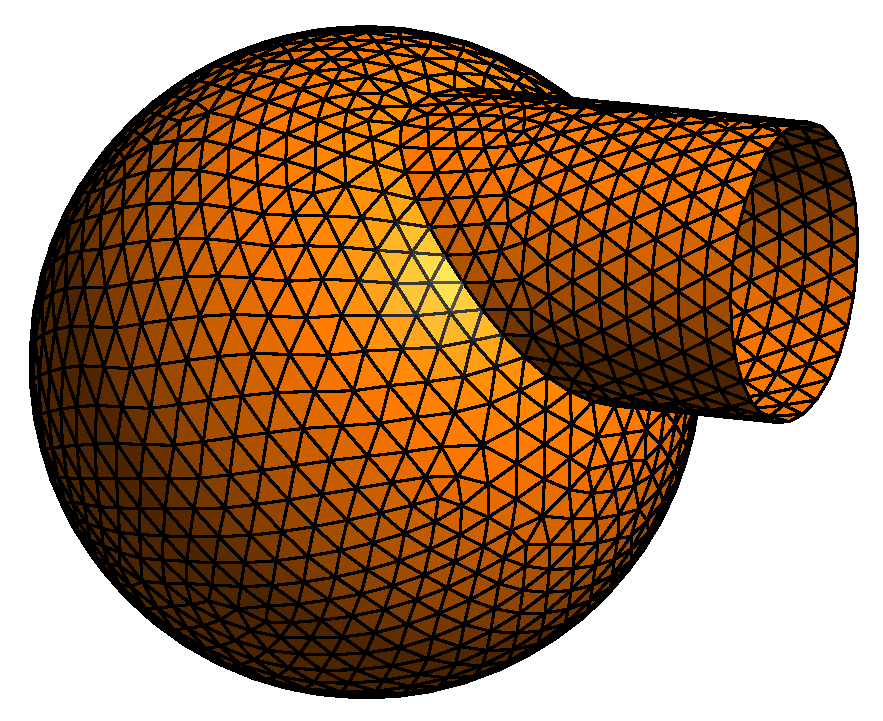
\includegraphics[width=80mm]{sphere-cyl}
  \caption{Sphere glued to cylinder}
  \label{\numb section 3.\numb fig 5}
\end{figure}

\begin{figure}[ht] \centering
 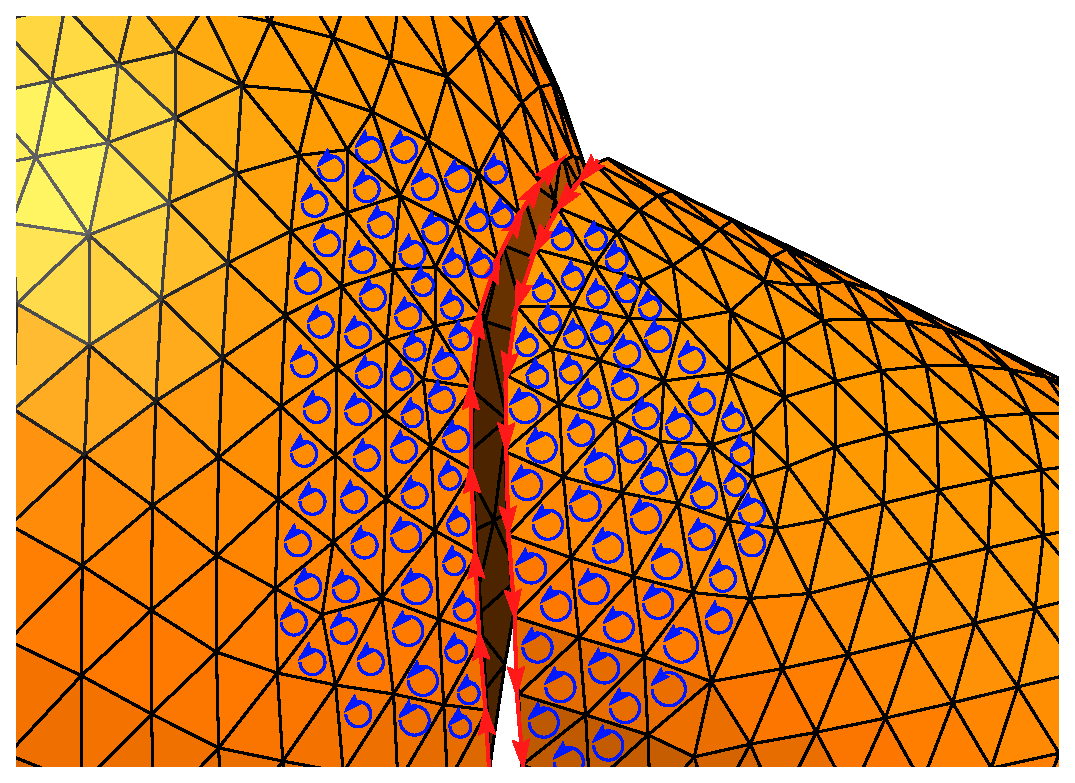
\includegraphics[width=100mm]{crack}
  \caption{Zoom around the joint}
  \label{\numb section 3.\numb fig 6}
\end{figure}

Note how the orientation is important (see paragraphs \ref{\numb section 1.\numb parag 2}
and \ref{\numb section 1.\numb parag 3}).
For meshing the piece of cylinder, we provide its future boundary which is the union of
{\small\tt circle\_\,1} with {\small\tt circle\_\,2.reverse()}.
For meshing the sphere, we provide {\small\tt circle\_\,2}.
In figure \ref{\numb section 3.\numb fig 6}, where a crack has been opened artificially,
we see that the common boundary has a certain orientation when seen from the cylinder and
has the opposite orientation when seen from the sphere.
If we do not respect these orientations, {\maniFEM} will be unable to {\small\tt join} the two
meshes.

If we want to close the extremity of the cylinder, it suffices to add a few lines of code$\,$:

\begin{Verbatim}[commandchars=\\\{\},formatcom=\small\tt,
   baselinestretch=0.94,framesep=2mm                     ]
   RR3.implicit ( x == 1.5 );
   \verm{Mesh} \azul{disk} ( \verm{tag}::progressive, \verm{tag}::boundary, circle_1.reverse(),
               \verm{tag}::start_at, start_1, \verm{tag}::towards, \{ 0., 0., -1. \},
               \verm{tag}::desired_length, seg_size                         );
   \verm{Mesh} \azul{sphere_and_cylinder} ( \verm{tag}::join, piece_of_sph, piece_of_cyl, disk );
\end{Verbatim}

We have chosen the diameter of the cylinder slightly smaller than $1$.
Had we chosen a diameter equal to $1$, the cylinder would be tangent to the sphere at point
$ (0,0,1) $.
At that point, the two equations defining the {\small\tt intersection} manifold would be
degenerate (the Jacobian matrix would not have full rank).
This is a situation which {\maniFEM} cannot handle yet; it is discussed in paragraph
\ref{\numb section 3.\numb parag 21}.


          %------------------%
\section{~~Sharp edges, again}\label{\numb section 3.\numb parag 19}
          %------------------%

With a few changes to the code in paragraph \ref{\numb section 3.\numb parag 18},
we can cut two holes in the sphere and create a tunnel using the cylinder's wall.
\medskip

\begin{figure}[ht] \centering
\if\production 1
 \includegraphics[width=94mm]{sphere-tunnel-cloud-im}
\else
 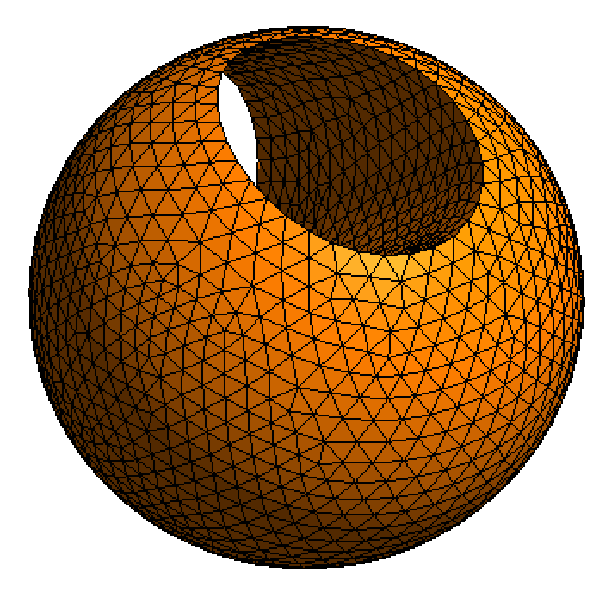
\includegraphics[width=94mm]{sphere-tunnel-low-res}
\fi
  \caption{Sphere with tunnel}
  \label{\numb section 3.\numb fig 7}
\end{figure}

\begin{Verbatim}[commandchars=\\\{\},formatcom=\small\tt,frame=single,
   label=parag-\ref{\numb section 3.\numb parag 19}.cpp,rulecolor=\color{coment},
   baselinestretch=0.94,framesep=2mm                                            ]
   \verm{Manifold} \azul{cylinder} = RR3.implicit ( y*y + (z-0.5)*(z-0.5) == rc*rc );
   \verm{Manifold} \azul{intersection} = cylinder.implicit ( x*x + y*y + z*z == rs*rs );
   \verm{Cell} \azul{start_1} ( \verm{tag}::vertex );
   x ( start_1 ) = 1.;  y ( start_1 ) = 0.;  z ( start_1 ) = 0.5 - rc;
   intersection.project ( start_1 );
   \verm{Mesh} \azul{circle_1} ( \verm{tag}::progressive, \verm{tag}::start_at, start_1,
                   \verm{tag}::towards, \{ 0., 1., 0. \}, \verm{tag}::desired_length, seg_size );
   \verm{Cell} \azul{start_2} ( \verm{tag}::vertex );
   x ( start_2 ) = -1.;  y ( start_2 ) = 0.;  z ( start_2 ) = 0.5 - rc;
   intersection.project ( start_2 );
   \verm{Mesh} \azul{circle_2} ( \verm{tag}::progressive, \verm{tag}::start_at, start_2,
                   \verm{tag}::towards, \{ 0., 1., 0. \}, \verm{tag}::desired_length, seg_size );
   \verm{Mesh} \azul{two_circles} ( \verm{tag}::join, circle_1.reverse(), circle_2 );
   cylinder.set_as_working_manifold();
   \verm{Mesh} \azul{piece_of_cyl} ( \verm{tag}::progressive, \verm{tag}::boundary, two_circles,
                       \verm{tag}::start:at, start_1, \verm{tag}::towards, \{ -1., 0., 0. \},
                       \verm{tag}::desired_length, seg_size                         );
   \verm{Mesh} \azul{two_circles_rev} ( \verm{tag}::join, circle_1, circle_2.reverse() );
   RR3.implicit ( x*x + y*y + z*z == rs*rs );
   \verm{Mesh} \azul{piece_of_sph} ( \verm{tag}::progressive, \verm{tag}::boundary, two_circles_rev,
                       \verm{tag}::start:at, start_1, \verm{tag}::towards, \{ 0., 0., -1. \},
                       \verm{tag}::desired_length, seg_size                         );
   \verm{Mesh} \azul{perf_sphere} ( \verm{tag}::join, piece_os_sph, piece_of_cyl );
\end{Verbatim}

{\ManiFEM} deals well with a disconnected manifold like {\small\tt intersection}.
Each of the constructors {\small\tt \verm{Mesh} circle\_\,1} and {\small\tt \verm{Mesh} circle\_\,2} meshes only
a connected component of {\small\tt intersection}, depending on the starting point we provide.

Had we chosen a cylinder of diameter $1$, a singular point would have appeared;
the two ``circles'' would touch at point $ (0,0,1) $.
This is a situation which {\maniFEM} cannot handle yet; it is discussed in paragraph
\ref{\numb section 3.\numb parag 21}.


                  %------------%
\section{~~\cinza{Singularities}}\label{\numb section 3.\numb parag 20}
                  %------------%

{\normalfont\bfseries The code described in this paragraph does not work yet.
It should be regarded as a mere declaration of intentions.}
\medskip

If we want to mesh (a part of) a surface with singular points, we must give to {\maniFEM}
knowledge about these singularities.
A typical example is the vertex of a cone.

\begin{figure}[ht] \centering
 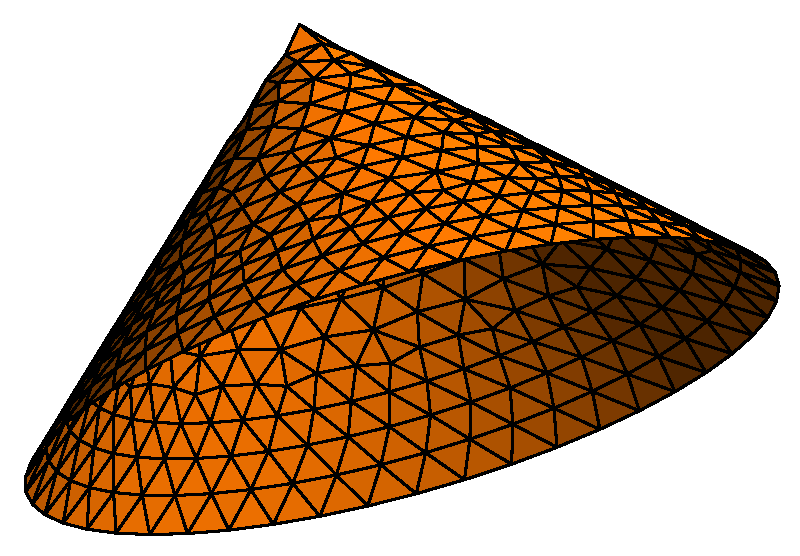
\includegraphics[width=85mm]{cone}
  \caption{A singularity (vertex)}
  \label{\numb section 3.\numb fig 8}
\end{figure}

\begin{Verbatim}[commandchars=\\\{\},formatcom=\small\tt,frame=single,
   label=code not working,rulecolor=\color{coment},
   baselinestretch=0.94,framesep=2mm                                  ]
   \verm{Manifold} \azul{cone_manif} = RR3.implicit ( x*x + y*x == z*z );
   cone_manif.implicit ( z == 1. );
   \verm{Cell} \azul{A} ( \verm{tag}::vertex );  x(A) = 1.;  y(A) = 0.;  z(A) = 1.;
   \verm{Mesh} \azul{circle} ( \verm{tag}::progressive, \verm{tag}::start_at, A,
                 \verm{tag}::towards, \{ 0., -1., 0. \},
                 \verm{tag}::desired_length, 0.1           );
   cone_manif.set_as_working_manifold();
   \verm{Cell} \azul{V} ( \verm{tag}::vertex );  x(V) = 0.;  y(V) = 0.;  z(V) = 0.;
   \verm{Mesh} \azul{cone} ( \verm{tag}::progressive, \verm{tag}::boundary, circle,
               \verm{tag}::start_at, A, \verm{tag}::towards, \{ -1., 0., -1. \},
               \verm{tag}::singular, V, \verm{tag}::desired_length, 0.1       );
\end{Verbatim}


                 %--------------------%
\section{~~\cinza{Singularities, again}}\label{\numb section 3.\numb parag 21}
                 %--------------------%

{\normalfont\bfseries The code described in this paragraph does not work yet.
It should be regarded as a mere declaration of intentions.}
\medskip

Besides vertices like the one described in paragraph \ref{\numb section 3.\numb parag 20},
another kind of singularity appears when we intersect two manifolds which have a tangency point.
This happens if we choose {\small\tt rc = 0.5} in paragraph \ref{\numb section 3.\numb parag 18}
or \ref{\numb section 3.\numb parag 19}.

We focus on the piece of cylinder from paragraph \ref{\numb section 3.\numb parag 19}
(which is to be subsequently {\small\tt join}ed with a sphere with two holes).

\begin{figure}[ht] \centering
 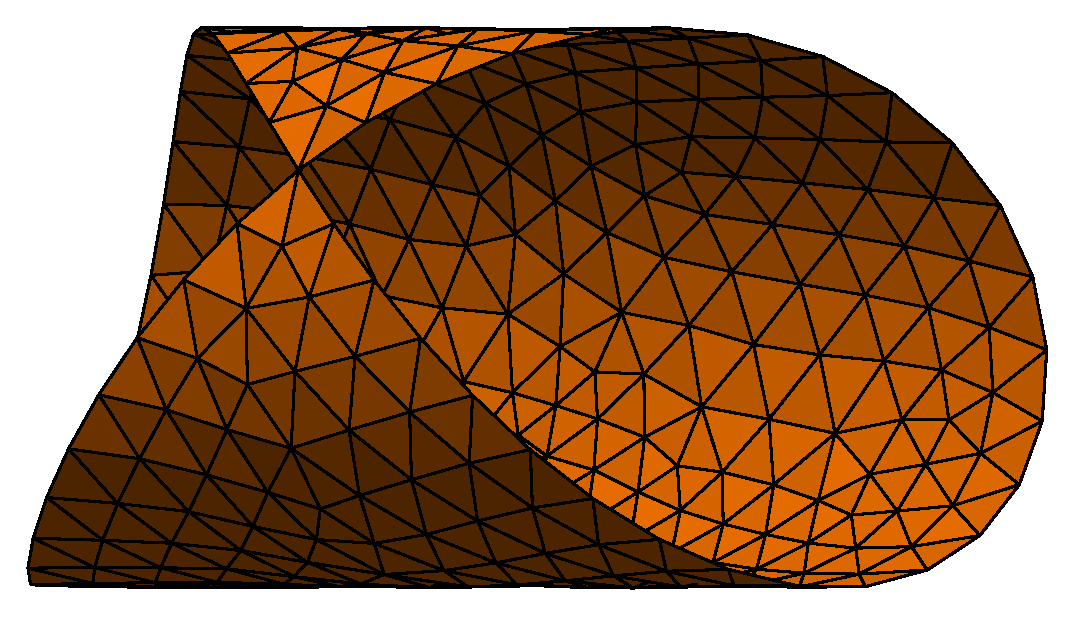
\includegraphics[width=85mm]{cyl}
  \caption{A singularity (napkin)}
  \label{\numb section 3.\numb fig 9}
\end{figure}

\begin{Verbatim}[commandchars=\\\{\},formatcom=\small\tt,frame=single,
   label=code not working,rulecolor=\color{coment},
   baselinestretch=0.94,framesep=2mm                                  ]
   \verm{Manifold} \azul{cylinder} = RR3.implicit ( y*y + (z-0.5)*(z-0.5) == 0.25 );
   \verm{Manifold} \azul{infinity} = cylinder.implicit ( x*x + y*y + z*z == 1. );
   \verm{Cell} \azul{V} ( \verm{tag}::vertex );  x(V) = 0.;  y(V) = 0.;  z(V) = 1.;
   \verm{Mesh} \azul{circle_1} ( \verm{tag}::progressive,
                   \verm{tag}:: start_at, V, \verm{tag}::towards, \{ 1., 1., 0. \},
                   \verm{tag}::singular, V, \verm{tag}::desired_length, 0.1      );
   \verm{Mesh} \azul{circle_2} ( \verm{tag}::progressive,
                   \verm{tag}:: start_at, V, \verm{tag}::towards, \{ -1., -1., 0. \},
                   \verm{tag}::singular, V, \verm{tag}::desired_length, 0.1        );

   cylinder.set_as_working_manifold();
   \verm{Cell} \azul{W} = circle_1.cell_in_front_of(V).tip();
   \verm{Mesh} \azul{piece_of_cyl} ( \verm{tag}::progressive, \verm{tag}::boundary, circle_1, circle_2,
                       \verm{tag}::start_at, W, \verm{tag}::towards, \{ -1., 1., 0. \},
                       \verm{tag}::singular, V, \verm{tag}::desired_length, 0.1          );
\end{Verbatim}

{\ManiFEM} accepts as {\small\tt \verm{Manifold}} a self-intersecting set like {\small\tt infinity}.
However, in the {\small\tt \verm{Mesh}} constructor we must specify {\small\tt V} as singular point.

Unlike in paragraph \ref{\numb section 3.\numb parag 19}, here we cannot {\small\tt join} the
two meshes {\small\tt circle\_\,1} and {\small\tt circle\_\,2}.
{\ManiFEM} is unable to join two closed polygonal lines having a vertex in common;
in other words, it does not handle self-intersecting {\small\tt \verm{Mesh}}es.
This is why we provide the two pieces of boundary separately.


          %-------------------%
\section{~~Non-uniform meshing}\label{\numb section 3.\numb parag 22}
          %-------------------%

The {\small\tt desired\_\,length} may be a non-constant function.

\begin{Verbatim}[commandchars=\\\{\},formatcom=\small\tt,frame=single,
   label=parag-\ref{\numb section 3.\numb parag 22}.cpp,rulecolor=\color{coment},
   baselinestretch=0.94,framesep=2mm                                            ]
   \verm{Function} \azul{d} = 0.03 + 0.04 * ( (x+0.3)*(x+0.3) + (y-0.9)*(y-0.9) );
   \verm{Manifold} \azul{circle} = RR2.implicit ( x*x + y*y == 1. );
   \verm{Mesh} \azul{outer} ( \verm{tag}::progressive, \verm{tag}::desired_length, d );
   \verm{Manifold} \azul{ellipse} = RR2.implicit ( x*x + (y-0.37)*(y-0.37) + 0.3*x*y == 0.25 );
   \verm{Mesh} \azul{inner} ( \verm{tag}::progressive, \verm{tag}::desired_length, d );
   \verm{Mesh} \azul{bdry} ( \verm{tag}::join, outer, inner.reverse() );
   RR2.set_as_working_manifold();
   \verm{Mesh} \azul{disk} ( \verm{tag}::progressive, \verm{tag}::boundary, bdry, \verm{tag}::desired_length, d );
\end{Verbatim}

\begin{figure}[ht] \centering
 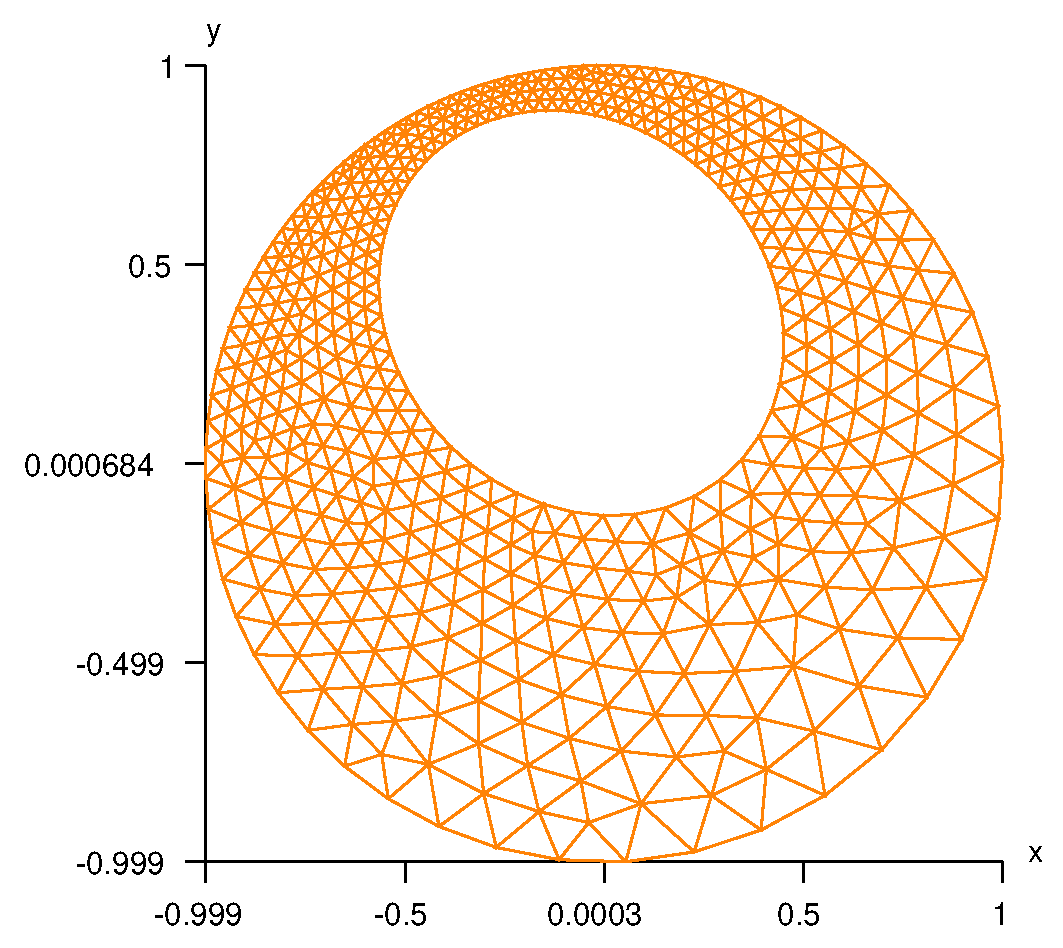
\includegraphics[width=90mm]{disk-non-unif}
  \caption{Non-uniform mesh}
  \label{\numb section 3.\numb fig 10}
\end{figure}

Compare with the mesh in paragraph \ref{\numb section 3.\numb parag 3}.

It is the user's responsibility to provide a {\small\tt desired\_\,length} which takes positive
values at all points of the future mesh.
Also, {\small\tt desired\_\,length} should be a reasonably smooth function;
sharp variations should be avoided.


                 %---------------------------%
\section{~~\cinza{Changing the Riemann metric}}\label{\numb section 3.\numb parag 23}
                 %---------------------------%
 
{\normalfont\bfseries The code described in this paragraph does not work yet.
It should be regarded as a mere declaration of intentions.}
\medskip

We can attach a non-uniform metric to our manifold; as a consequence, for a constant
{\small\tt desired\_\,length}, the apparent segment length will vary from zone to zone.
For instance, in the code below we set a metric which increases the measured length
of the segments close to the narrow part of the domain.
As a consequence, the meshing algorithm, while trying to build a mesh of constant
{\small\tt desired\_\,length}, will choose shorter segments in the proximity of the narrow zone
(because the length measured by the Riemann metric will be larger than the length
we see in the drawing), thus producing the same result as in paragraph
\ref{\numb section 3.\numb parag 22}.

\begin{Verbatim}[commandchars=\\\{\},formatcom=\small\tt,frame=single,
   label=code not working,rulecolor=\color{coment},
   baselinestretch=0.94,framesep=2mm                                   ]
   \verm{Manifold} \azul{RR2} ( \verm{tag}::Euclid, \verm{tag}::of_dim, 2 );
   \verm{Function} \azul{xy} = RR2.build_coordinate_system ( \verm{tag}::Lagrange, \verm{tag}::of_degree, 1 );
   \verm{Function} \azul{x} = xy[0],  \azul{y} = xy[1];
   \verm{Function} \azul{d} = 0.3 + 0.5 * ( (x+0.3)*(x+0.3) + (y-0.9)*(y-0.9) );
   RR2.set_metric ( 1. / d );
   
   \verm{Manifold} \azul{circle} = RR2.implicit ( x*x + y*y == 1. );
   \verm{Mesh} \azul{outer} ( \verm{tag}::progressive, \verm{tag}::desired_length, 0.1 );
   \verm{Manifold} \azul{ellipse} = RR2.implicit ( x*x + (y-0.37)*(y-0.37) + 0.3*x*y == 0.25 );
   \verm{Mesh} \azul{inner} ( \verm{tag}::progressive, \verm{tag}::desired_length, 0.1 );
   \verm{Mesh} \azul{bdry} ( \verm{tag}::join, outer, inner.reverse() );
   RR2.set_as_working_manifold();
   \verm{Mesh} \azul{disk} ( \verm{tag}::progressive, \verm{tag}::boundary, bdry, \verm{tag}::desired_length, 0.1 );
\end{Verbatim}

These two approaches (the one described in paragraph \ref{\numb section 3.\numb parag 22} and
the one described here) can be used interchangeably.
It is possible to use both in the same code, but the code will become rather obscure.


                 %------------------%
\section{~~\cinza{Anisotropic metric}}\label{\numb section 3.\numb parag 24}
                 %------------------%

{\normalfont\bfseries The code described in this paragraph does not work yet.
It should be regarded as a mere declaration of intentions.}
\medskip

The technique described in paragraph \ref{\numb section 3.\numb parag 23} can be generalized to
an anisotropic Riemann metric.
We define the metric by means of a square matrix $M$.
$M$ must be symmetric positive definite.
The arguments of {\small\tt set\_\,metric} are $ m_{11} $, $ m_{12} $ and $ m_{22} $
for two dimensions,
$ m_{11} $, $ m_{12} $, $ m_{13} $, $ m_{22} $, $ m_{23} $ and $ m_{33} $ for three dimensions.

\begin{Verbatim}[commandchars=\\\{\},formatcom=\small\tt,frame=single,
   label=code not working,rulecolor=\color{coment},
   baselinestretch=0.94,framesep=2mm                                  ]
   \verm{Manifold} \azul{RR2} ( \verm{tag}::Euclid, \verm{tag}::of_dim, 2 );
   \verm{Function} \azul{xy} = RR2.build_coordinate_system ( \verm{tag}::Lagrange, \verm{tag}::of_degree, 1 );
   \verm{Function} \azul{x} = xy[0],  \azul{y} = xy[1];
   \verm{Function} \azul{d} = 0.3 + (x+0.3)*(x+0.3) + (y-0.9)*(y-0.9);
   RR2.set_metric ( 1. + 1./d, -3./d, 1. + 9./d );
   \cinza{// or, equivalently :}
   \cinza{// RR2.set_metric ( tag::principal_part, 1.,}
   \cinza{//                  tag::deviatoric_part, 1./d, -3./d, 9./d );}

   \verm{Manifold} \azul{circle} = RR2.implicit ( x*x + y*y == 1. );
   \verm{Mesh} \azul{outer} ( \verm{tag}::progressive, \verm{tag}::desired_length, 0.1 );
   \verm{Manifold} \azul{ellipse} = RR2.implicit ( x*x + (y-0.37)*(y-0.37) + 0.3*x*y == 0.25 );
   \verm{Mesh} \azul{inner} ( \verm{tag}::progressive, \verm{tag}::desired_length, 0.1 );
   \verm{Mesh} \azul{bdry} ( \verm{tag}::join, outer, inner.reverse() );
   RR2.set_as_working_manifold();
   \verm{Mesh} \azul{disk} ( \verm{tag}::progressive, \verm{tag}::boundary, bdry, \verm{tag}::desired_length, 0.1 );
\end{Verbatim}

\begin{figure} \centering
 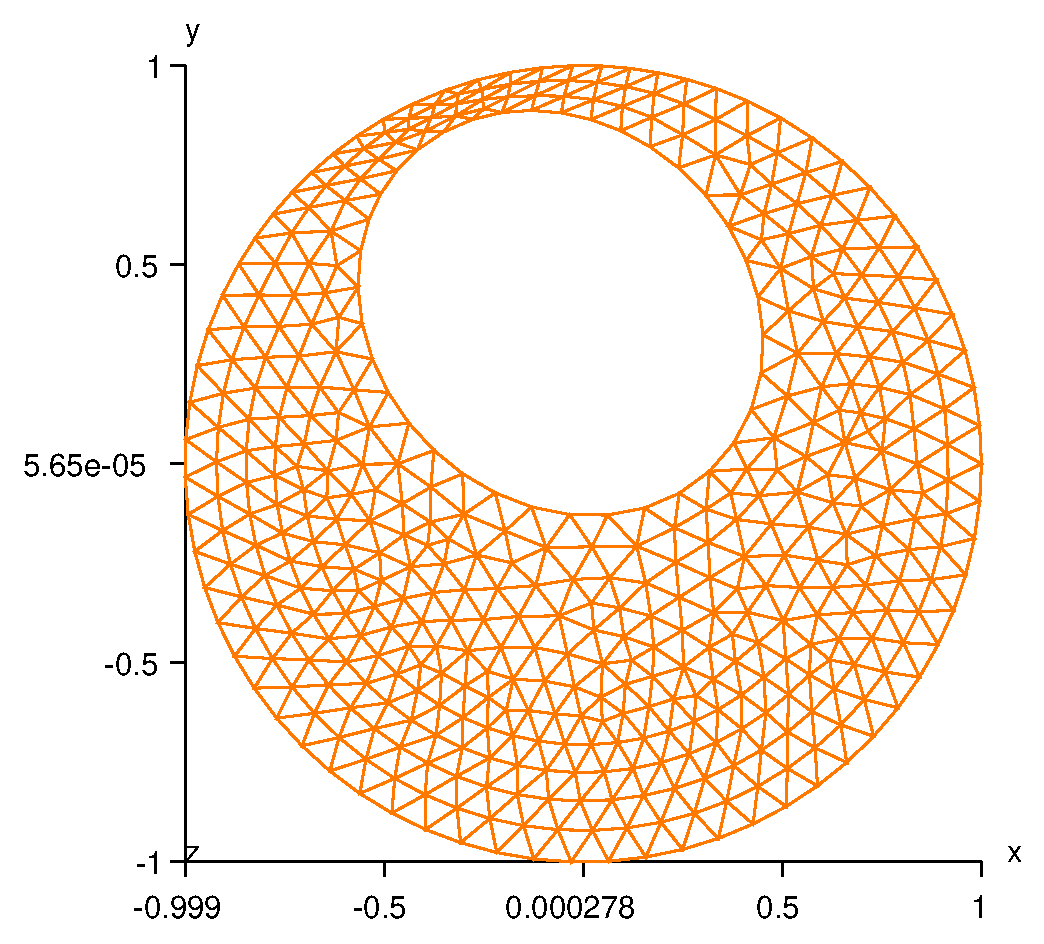
\includegraphics[width=90mm]{disk-anisotrop}
  \caption{Anisotropic mesh}
  \label{\numb section 3.\numb fig 11}
\end{figure}

Compare with the mesh in paragraph \ref{\numb section 3.\numb parag 3}.

This result cannot be achieved using the approach of paragraph
\ref{\numb section 3.\numb parag 22} (by setting a non-constant {\small\tt desired\_\,length}).


          %-----------%
\section{~~Future work}\label{\numb section 3.\numb parag 25}
          %-----------%

It would be nice to define domains using inequalities between {\small\tt \verm{Function}}s.

